\chapter{Implementasi dan Pengujian}
\label{chap:implementasiDanPengujian}

Pada bab ini dijelaskan mengenai implementasi dari seluruh hasil analisis dan perancangan yang telah dilakukan pada bab-bab sebelumnya dan pengujian yang dilakukan untuk hasil implementasi tersebut. Hasil pengujian akan digunakan untuk mengukur performansi dan kualitas dari perangkat lunak yang dibuat.

\section{Implementasi}
\label{sec:implementasi}

Pada subbab \ref{sec:DiagramKelasLengkap} telah dirancang beberapa kelas yang menjadi bagian dari perangkat lunak morphological parser. Implementasi dari kelas-kelas tersebut menjadi sebuah perangkat lunak akan dilakukan dengan menggunakan bahasa pemrograman Java. Implementasi meliputi keseluruhan method dan atribut untuk setiap kelas yang sudah dirancang. Pada kelas Lexicon dan Node, terdapat atribut yang memiliki tipe map of Node dengan key sebuah karakter, atribut ini diimplementasikan dengan hash table pada kelas HashMap yang dimiliki oleh bahasa Java.

Penyimpanan leksikon, seperti dibahas pada subbab \ref{sec:strukturPenyimpananLeksikon}, dilakukan dalam file khusus berekstensi '.lxc'. Supaya perangkat lunak dapat melakukan proses baca dan tulis dari dan ke file tersebut, diperlukan suatu implementasi dari proses baca tulis file oleh perangkat lunak. Proses ini diimplementasikan dalam bahasa Java dengan kelas BufferedReader dan kelas BufferedWriter yang menggunakan objek Reader dari kelas FileReader dan kelas FileWriter.

Untuk implementasi dari rancangan antarmuka perangkat lunak, dilakukan dengan menggunakan kelas JFrame dalam bahasa Java. Sebagai tambahan dari perancangan yang sudah dilakukan, ditambahkan fitur untuk mengaktifkan dan mematikan fitur validator dan converter dari perangkat lunak. Fitur validator adalah fitur untuk melakukan validasi hasil parsing pada kata turunan dalam leksikon, seperti yang dibahas pada subbab \ref{sec:leksikon}. Sementara fitur converter adalah fitur untuk melakukan konversi hasil parsing dari simbol leksikon menjadi kata-kata yang dapat dimengerti oleh manusia. Gambar \ref{gambar-implementasi-antarmuka} berikut adalah implementasi antarmuka untuk perangkat lunak morphological parser.

\begin{figure}[H]
\centering
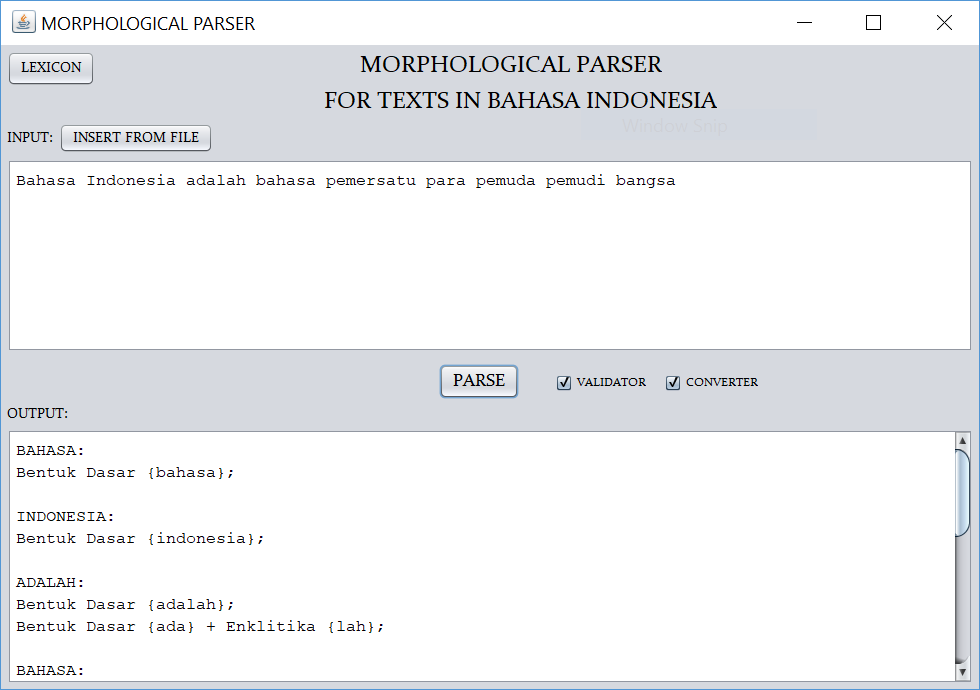
\includegraphics[scale=0.7]{Gambar/gambar-implementasi-antarmuka}
\caption{Implementasi antarmuka perangkat lunak morphological parser} 
\label{gambar-implementasi-antarmuka}
\end{figure}

\section{Pengujian}
\label{sec:pengujian}

\subsection{Pengujian Fungsional}
\label{sec:pengujianFungsional}

\subsection{Pengujian Nonfungsional}
\label{sec:pengujianNonfungsional}

Jangan lupa kesimpulan pengujian